\documentclass[dvipdfmx,11pt]{beamer}

\usetheme{Madrid}
\usefonttheme{professionalfonts}

\definecolor{tohokuPurple}{RGB}{62,21,134}
\setbeamercolor{structure}{fg=tohokuPurple}
\setbeamercolor{frametitle}{bg=tohokuPurple, fg=white}

\setbeamercolor{title}{fg=white, bg=tohokuPurple}
\setbeamercolor{author}{fg=black}
\setbeamercolor{institute}{fg=black}
\setbeamercolor{date}{fg=black}

\setbeamercolor{block title}{bg=tohokuPurple, fg=white}
\setbeamercolor{block body}{bg=tohokuPurple!5, fg=black}
\setbeamertemplate{navigation symbols}{}

\usepackage{amsmath,amssymb,bm}
\usepackage{listings,booktabs}
\usepackage{graphicx}
\graphicspath{{../figures/}{figures/}}
\usepackage{tikz}
\usetikzlibrary{arrows.meta,positioning}
\usepackage{hyperref}
\usepackage{bookmark}

\title{解釈可能な深層VARの提案}
\author[栗田 煌矢]{
  東北大学経済学部4年李研\texorpdfstring{\\}{ }\
  栗田 煌矢}

\date{\today}

\begin{document}

\begin{frame}
  \titlepage
\end{frame}


\begin{frame}{多変量時系列解析}

 

VAR(ベクトル自己回帰)モデルは、複数の時系列データの相互依存関係を表現するためのモデルである。
  \[
    x_t
    =
    \sum_{k=1}^{K}
    \Phi_k x_{t-k}
    +
    \varepsilon_t
  \]

$x_t$は時点$t$の多変量ベクトル、$\Phi_k$はラグ$k$に対応する係数行列。
  
本研究はVARに代表される多変量時系列解析がテーマとなる。

\end{frame}



\begin{frame}{提案手法について}

  \begin{enumerate}
    \item GVARにより、状態依存的かつ符号解釈が可能な係数行列を学習する。
    \item Neural Granger Causality型の正則化により、係数行列を効果的にスパース化する。
    \item 学習可能な\texttt{causal\_gate}に近接勾配法を適用し、係数行列の厳密なゼロと、自動ラグ選択を実現。
  \end{enumerate}
\end{frame}

\begin{frame}{提案手法について}
  \small
  次を同時に満たす点が特徴であり、貢献であると考える。

  \vspace{0.4em}
  \begin{enumerate}
    \item \textbf{非線形・状態依存性}：時点ごとに変化する効果を表現できる。
    \item \textbf{構造スパース性}：存在しない変数間関係を厳密なゼロとして除去できる。
    \item \textbf{係数としての解釈性}：ラグ、符号、効果の大きさを読み取れる。
  \end{enumerate}

  \vspace{0.5em}
  \scriptsize
  \setlength{\tabcolsep}{4pt}
  \renewcommand{\arraystretch}{1.25}
  \center
  \begin{tabular}{@{}lccc@{}}
    \toprule
    手法 & 非線形・状態依存 & 厳密な構造スパース性 & 係数の解釈 \\
    \midrule
    VAR & × & ○ & ○ \\
    LSTM & ○ & × & × \\
    NGC & ○ & ○ & ×\\
    GVAR & ○ & × & ○ \\
    \textbf{本研究} & \textbf{○} & \textbf{○} & \textbf{○} \\
    \bottomrule
  \end{tabular}

  \vspace{0.6em}
  \normalsize
\textbf{非線形のわりにはリッチな解釈をシンプルに行えるモデルを目指した。}
\end{frame}


\begin{frame}{背景：GVARとNeural Granger Causality}
  提案手法は、次の2つの既存手法をcausal gateで統合している。

  \begin{enumerate}
    \item GVAR：状態依存的で符号解釈が可能な係数行列をニューラルネットワークで生成する(Marcinkevičs, R., \& Vogt, J. E.,2021)。
    \item Neural-GC：ニューラルネットワークに構造的スパース性を導入し、Granger因果性を推定する(Tank et al.,2021)。
  \end{enumerate}

  \vspace{0.5em}

  \[
    \texttt{causal\_gate.shape} = [\text{lag}, \text{target}, \text{source}]
  \]
\end{frame}

\begin{frame}{提案手法の全体像}
\centering
\small
\resizebox{0.98\linewidth}{!}{%
\begin{tikzpicture}[
  node distance=0.75cm and 0.8cm,
  box/.style={draw, rounded corners, align=center, minimum width=2.45cm, minimum height=0.8cm},
  gate/.style={draw, rounded corners, align=center, minimum width=2.45cm, minimum height=0.8cm, fill=blue!8},
  op/.style={draw, circle, inner sep=1.5pt},
  sumop/.style={draw, circle, inner sep=2pt, fill=gray!8},
  arr/.style={-Latex, thick}
]
  \node[box] (input) {ラグ付き入力\\$x_{t-K:t-1}$};
  \node[box, right=of input] (coefnet) {係数出力モデル\\NNなど};
  \node[box, right=of coefnet] (phi) {状態依存係数\\$\Phi_{k(x_{t-k})}$};
  \node[gate, below=of phi] (gate) {causal gate\\$G_k$};
  \node[op, right=of phi] (prod) {$\odot$};
  \node[box, right=of prod] (eff) {有効係数\\$\tilde{\Phi}_{k,t}$};
  \node[op, right=of eff] (mprod) {$\times$};
  \node[box, right=of mprod] (pred) {予測値\\$\hat{x}_t$};


  \draw[arr] (input) -- (coefnet);
  \draw[arr] (coefnet) -- (phi);
  \draw[arr] (phi) -- (prod);
  \draw[arr] (gate) -| (prod);
  \draw[arr] (prod) -- (eff);
  \draw[arr] (eff) -- (mprod);
  \draw[arr] (input.north) to[out=70,in=115,looseness=0.35] (mprod.north);
  \draw[arr] (mprod) -- (pred);

  \node[align=center, below=0.25cm of gate] {\scriptsize 近接勾配法で\\[-0.1em]\scriptsize 厳密ゼロ化};
\end{tikzpicture}
}

\vspace{0.6em}
\[
  \tilde{\Phi}_{k,t}
  =
  G_k \odot \Phi_{k(x_{t-k})},
  \qquad
  \hat{x}_t
  =
  \sum_{k=1}^{K}
  \tilde{\Phi}_{k,t} x_{t-k}
\]
\end{frame}

\begin{frame}{GVAR(Marcinkevičs, R., \& Vogt, J. E.,2021)}
  $p$変量時系列を
  \[
    x_t = (x_{t,1}, \ldots, x_{t,p})^\top \in \mathbb{R}^{p}
  \]
  とする。自己回帰次数を$K$とすると、一般化VAR(GVAR)は次のように表される。

  \[
    x_t
    =
    \sum_{k=1}^{K}
    \Phi_{k(x_{t-k})} x_{t-k}
    +
    \varepsilon_t
  \]

  $\Phi_{k(x_{t-k})} \in \mathbb{R}^{p \times p}$はラグ$k$に対応する
  \textbf{状態依存的}な係数行列であり、これがニューラルネットの出力となる。
    
  \vspace{1.0em}
  \begin{center}
    \textbf{特徴}：係数の符号解釈が可能であるが、事後的な閾値処理が必要。
  \end{center}

  
\end{frame}


\begin{frame}{Neural Granger Causality (NGC) (Tank et al.,2021)}
  
  NNのスパース制約を工夫し、Granger因果性を推定する手法である。

  \vspace{0.5em}
  \begin{block}{Theorem (Tank et al.,2021)}
    変数$j$が変数$i$をGranger causeしないための十分条件は、
    すべてのラグにおいて$j$から$i$への重みがゼロであることである。
  \end{block}
  この条件を満たすように、\textbf{入力層重みに対して構造的な厳密スパース最適化(近接勾配法)}を行う。

  \vspace{1.0em}

  \begin{center}
    \textbf{特徴}：事後的な閾値処理はいらないが、係数の符号は意味を持たない。
  \end{center}
\end{frame}



\begin{frame}{Causal Gateによる構造制御}
 ラグごとの係数行列それぞれに対してcausal gateを適用。
 最終的な係数行列は次で定義される。

  \[
    \tilde{\Phi}_{k(x_{t-k})}
    =
    G_k \odot \Phi_{k(x_{t-k})} 
    \quad , \quad  
    G_k \in \mathbb{R}^{p \times p}
  \]
  \vspace{0.5em}
  動的な係数変動は$\Phi_{k(x_{t-k})}$が表現し、全体としてのGranger因果の有無を$G_k$が制御するという役割の分離。

  \vspace{0.5em}
  \center
    \textbf{本研究ではこのgateに構造スパース制約をかけることでGranger因果性を推定する。}
\end{frame}

\begin{frame}{Causal Gateの狙い}
  係数$\Phi_{k(x_{t-k})}$は入力値依存であるため、
  同じラグの入力なのに値によって係数が0になる場合とならない場合がある。

  \vspace{0.5em}
  入力に依存しない\texttt{causal\_gate}を設け、構造スパース化をかけることで
  \[
    G_{1,i,j}=\cdots=G_{K,i,j}=0
  \]
  なら、任意の入力に対して$j \to i$の有効係数は0。

  \vspace{0.5em}
  入力値依存性に惑わされず、gateのみで因果性を解釈できる。
\end{frame}


\begin{frame}{本研究のGranger非因果性の定義}
  変数$x_j$が変数$x_i$をGranger causeしないための十分条件は、
  すべてのラグにおいて$x_j$から$x_i$への効果がゼロであることである。
  つまり、
  \[
    G_{1,i,j} = G_{2,i,j} = \cdots = G_{K,i,j} = 0
  \]

  causal gateの値が全てのラグにおいて0であれば、
  最終的な係数行列$\tilde{\Phi}_k(x_{t-k})$は、どんな入力値であろうと0になる。

  したがって、非因果性を主張するためには、gateの値を厳密な0にする工夫が必要である。
\end{frame}




\begin{frame}{目的関数}
  予測損失、時間方向の平滑化、NGC正則化からなる。

  \[
    \mathcal{L}
    =
    \mathcal{L}_{\mathrm{pred}}
    +
    \mathcal{R}_{\mathrm{smooth}}
    +
    \mathcal{R}_{\mathrm{ngc}}
  \]

  \vspace{0.3em}

  予測損失は平均二乗誤差である。

  \[
    \mathcal{L}_{\mathrm{pred}}
    =
    \frac{1}{N}
    \sum_t
    \left\|
      x_t - \hat{x}_t
    \right\|_2^2
  \]

\end{frame}


\begin{frame}{Temporal Smoothness}
  状態依存係数を用いるため、係数が過度に振動しないための平滑化ペナルティ；

  \[
    \mathcal{R}_{\mathrm{smooth}}
    =
    \frac{\lambda_{\mathrm{smooth}}}{|\mathcal{T}|}
    \sum_{t \in \mathcal{T}}
    \left\|
      \tilde{\Phi}_{t+1}
      -
      \tilde{\Phi}_t
    \right\|_F^2
  \]

 同じ変数でもラグをまたいで大きく係数の値(or 符号)が変わるという
 不自然な動きを抑制し、過学習防止や解釈の妥当性を実現する。
\end{frame}

\begin{frame}{NGC型正則化：Sparse Group Lasso}
  \small
  Sparse Group Lassoは、特定の変数のエッジをすべてのラグでまとめて0にする圧力と、特定のラグの特定の変数のエッジを0にする圧力の両方を与える。

  \vspace{0.3em}
  \centering
  \resizebox{0.85\linewidth}{!}{%
  \begin{tikzpicture}[
    cell/.style={draw, rounded corners, minimum width=1.45cm, minimum height=0.72cm, align=center, fill=blue!8},
    note/.style={align=center},
    arr/.style={-Latex, thick}
  ]
    \node[note] at (-1.4,0) {edge\\$j \to i$};
    \node[cell] (g1) at (0.7,0) {$G_{1,i,j}$};
    \node[cell] (g2) at (2.25,0) {$G_{2,i,j}$};
    \node[cell] (dots) at (3.8,0) {$\cdots$};
    \node[cell] (gk) at (5.35,0) {$G_{K,i,j}$};

    \draw[very thick, blue!70!black] (-0.1,0.6) -- (6.15,0.6);
    \node[note, text=blue!70!black] at (3.0,1.05)
      {\scriptsize group lasso：edge全体をまとめて縮小};
    \draw[arr, blue!70!black] (3.0,0.9) -- (3.0,0.63);

    \foreach \x in {0.7,2.25,5.35} {
      \draw[arr, red!70!black] (\x,-0.75) -- (\x,-0.39);
    }
    \node[note, text=red!70!black] at (3.0,-1.1)
      {\scriptsize lasso：各lagのgateを個別に縮小};
  \end{tikzpicture}
  }

  \vspace{0.4em}
  \[
    \mathcal{R}_{\mathrm{SGL}}(G)
    =
    \lambda_{\mathrm{group}}
    \sum_{i,j}\|G_{:,i,j}\|_2
    +
    \lambda_{\mathrm{sparse}}
    \sum_{k,i,j}|G_{k,i,j}|
  \]
  \vspace{-0.4em}
  \scriptsize
  第1項はedge単位の削除、第2項はlag単位の削除を促す。
\end{frame}

\begin{frame}{NGC型正則化：Hierarchical Group Lasso}
  \small
  Hierarchical Group Lassoは古いラグに対応するgateの要素を
  優先的にゼロにする圧力をかけ、ラグの自動選択を実現する。

  \vspace{0.3em}
  \centering
  \resizebox{0.86\linewidth}{!}{%
  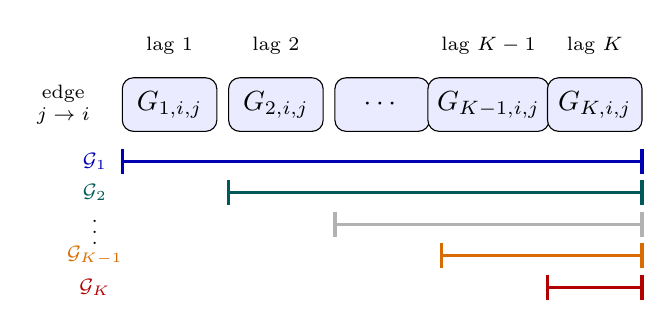
\begin{tikzpicture}[
    cell/.style={draw, rounded corners, minimum width=1.2cm, minimum height=0.68cm, align=center, fill=blue!8},
    note/.style={align=center, font=\scriptsize},
    brace/.style={very thick},
  ]
    \node[note] at (-1.35,0) {edge\\$j \to i$};
    \node[cell] (g1) at (0,0) {$G_{1,i,j}$};
    \node[cell] (g2) at (1.35,0) {$G_{2,i,j}$};
    \node[cell] (dots) at (2.7,0) {$\cdots$};
    \node[cell] (gkm) at (4.05,0) {$G_{K-1,i,j}$};
    \node[cell] (gk) at (5.4,0) {$G_{K,i,j}$};

    \node[font=\scriptsize] at (0,0.75) {lag 1};
    \node[font=\scriptsize] at (1.35,0.75) {lag 2};
    \node[font=\scriptsize] at (4.05,0.75) {lag $K-1$};
    \node[font=\scriptsize] at (5.4,0.75) {lag $K$};

    \node[note, text=blue!70!black] at (-0.95,-0.72) {$\mathcal{G}_{1}$};
    \draw[brace, blue!70!black] (-0.6,-0.72) -- (6.0,-0.72);
    \draw[brace, blue!70!black] (-0.6,-0.56) -- (-0.6,-0.88);
    \draw[brace, blue!70!black] (6.0,-0.56) -- (6.0,-0.88);

    \node[note, text=teal!70!black] at (-0.95,-1.12) {$\mathcal{G}_{2}$};
    \draw[brace, teal!70!black] (0.75,-1.12) -- (6.0,-1.12);
    \draw[brace, teal!70!black] (0.75,-0.96) -- (0.75,-1.28);
    \draw[brace, teal!70!black] (6.0,-0.96) -- (6.0,-1.28);

    \node[note] at (-0.95,-1.52) {$\vdots$};
    \draw[brace, gray!60] (2.1,-1.52) -- (6.0,-1.52);
    \draw[brace, gray!60] (2.1,-1.36) -- (2.1,-1.68);
    \draw[brace, gray!60] (6.0,-1.36) -- (6.0,-1.68);

    \node[note, text=orange!85!black] at (-0.95,-1.92) {$\mathcal{G}_{K-1}$};
    \draw[brace, orange!85!black] (3.45,-1.92) -- (6.0,-1.92);
    \draw[brace, orange!85!black] (3.45,-1.76) -- (3.45,-2.08);
    \draw[brace, orange!85!black] (6.0,-1.76) -- (6.0,-2.08);

    \node[note, text=red!70!black] at (-0.95,-2.32) {$\mathcal{G}_{K}$};
    \draw[brace, red!70!black] (4.8,-2.32) -- (6.0,-2.32);
    \draw[brace, red!70!black] (4.8,-2.16) -- (4.8,-2.48);
    \draw[brace, red!70!black] (6.0,-2.16) -- (6.0,-2.48);
  \end{tikzpicture}
  }

  \vspace{0.25em}
  \[
    \mathcal{G}_{k,i,j}
    =
    (G_{k,i,j},\ldots,G_{K,i,j}),
    \qquad
    \mathcal{R}_{\mathrm{HGL}}(G)
    =
    \lambda_{\mathrm{ngc}}
    \sum_{i,j}
    \sum_{k=1}^{K}
    \|\mathcal{G}_{k,i,j}\|_2
  \]

\end{frame}

\begin{frame}{Optimizer；近接勾配法(ISTA)}
ISTAは正則化で0に近づいたパラメータを、厳密に0にするための手法である。
ISTAでは次の2段階で\texttt{causal\_gate}を更新する。
\begin{center}
  \begin{enumerate}
    \item 予測損失と平滑化項に通常の勾配更新
    \item 更新後のgateを近接更新
  \end{enumerate}
\end{center}
 
  \[
    \text{勾配更新}
    \quad \longrightarrow \quad
    \text{近接更新}
    \quad \longrightarrow \quad
    G_{k,i,j}=0
  \]

  \vspace{0.6em}
  ここで使う超パラメータは、
  \[
    \eta \lambda
  \]
  であり、\textbf{モデルのパラメータ自体を0にする収縮圧力の強さ}をあらわす。

\end{frame}

\begin{frame}{事後的な閾値処理との違い}

  \vspace{0.55em}
  \begin{block}{比較}
    \begin{itemize}
      \item 近接勾配法で係数値が厳密に0になった変数は、モデル学習での推論過程に使われていない。
      \item 事後的な閾値処理では、学習中に小さい非ゼロ値の変数が推論過程に使われる。
    \end{itemize}
  \end{block}
  \vspace{1.5em}
   事後的な閾値処理でGranger非因果性を主張しても、モデル学習には微小に使われてしまっていることになるため
   近接勾配法などで学習中に厳密に0にすることが望ましい。
    
\end{frame}



\begin{frame}{解釈}
  \small
  \begin{block}{学習後の解釈}
    \begin{enumerate}
      \item causal gateからのGranger因果行列$\hat{A}$
      \item 有効係数$\tilde{\Phi}_{k,t}$
    \end{enumerate}
  \end{block}
  \vspace{0.2em}
  \centering
  \resizebox{0.96\linewidth}{!}{%
  \begin{tikzpicture}[
    cell/.style={draw, minimum size=0.62cm, inner sep=0pt, align=center, font=\scriptsize},
    gatecell/.style={cell, fill=blue!7},
    selected/.style={cell, fill=orange!35, draw=orange!85!black, very thick},
    outcell/.style={cell, fill=green!12},
    outselected/.style={cell, fill=orange!35, draw=orange!85!black, very thick},
    arr/.style={-Latex, thick}
  ]
    \foreach \x/\lag in {0/1,2.65/2,5.3/3} {
      \node[font=\scriptsize] at (\x+0.62,0.86) {lag \lag};
      \foreach \r/\y in {1/0,2/-0.62,3/-1.24} {
        \foreach \c/\xx in {1/0,2/0.62,3/1.24} {
          \node[gatecell] at (\x+\xx,\y) {};
        }
      }
      \node[selected] at (\x+1.24,-0.62) {};
      \node at (\x+1.24,-0.62) {\scalebox{0.62}{$G_{\lag,2,3}$}};
      \node[font=\scriptsize] at (\x, -1.78) {$x_1$};
      \node[font=\scriptsize] at (\x+0.62, -1.78) {$x_2$};
      \node[font=\scriptsize] at (\x+1.24, -1.78) {$x_3$};
      \node[font=\scriptsize] at (\x+0.62, -2.12) {source};
    }

    \node[font=\scriptsize, rotate=90] at (-1.25,-0.62) {target};
    \node[font=\scriptsize] at (-0.58,0) {$x_1$};
    \node[font=\scriptsize] at (-0.58,-0.62) {$x_2$};
    \node[font=\scriptsize] at (-0.58,-1.24) {$x_3$};

    \draw[arr] (7.35,-0.62) -- (8.7,-0.62)
      node[midway, above, font=\tiny] {lag方向に集約};

    \foreach \r/\y in {1/0,2/-0.62,3/-1.24} {
      \foreach \c/\xx in {1/0,2/0.62,3/1.24} {
        \node[outcell] at (10.0+\xx,\y) {};
      }
    }
    \node[outselected] at (11.24,-0.62) {};
    \node at (11.24,-0.62) {\scalebox{0.68}{$\hat{A}_{2,3}$}};
    \node[font=\scriptsize] at (10.62,0.86) {Granger因果行列 $\hat{A}$};
    \node[font=\scriptsize] at (10.0,-1.78) {$x_1$};
    \node[font=\scriptsize] at (10.62,-1.78) {$x_2$};
    \node[font=\scriptsize] at (11.24,-1.78) {$x_3$};
    \node[font=\scriptsize] at (10.62,-2.12) {source};
    \node[font=\scriptsize, rotate=90] at (9.0,-0.62) {target};
    \node[font=\scriptsize] at (9.42,0) {$x_1$};
    \node[font=\scriptsize] at (9.42,-0.62) {$x_2$};
    \node[font=\scriptsize] at (9.42,-1.24) {$x_3$};
  \end{tikzpicture}
  }

  \vspace{0.4em}
  \[
    g_{i,j}
    =
    (G_{1,i,j},G_{2,i,j},G_{3,i,j}),
    \qquad
    \hat{A}_{i,j}
    =
    \mathbf{1}
    \left[
      \|g_{i,j}\|_2 > \tau
    \right]
  \]

  \vspace{-0.4em}
  \center
  \scriptsize
  \begin{itemize}
    \item $\hat{A}_{i,j}=0$なら、変数$j$の過去が変数$i$の予測に寄与しないと判定する。
    \item 有効係数$\phi_{k,t}$の符号を見れば、目的変数への効果の方向を解釈できる。
  \end{itemize}
 
\end{frame}

\begin{frame}{実験設計}
\small

次の3点を、検証する。
\begin{enumerate}
  \item 閾値を置かずにGranger因果グラフを得られるか
  \item 真のGranger因果構造をどのとらえるか
  \item 状態依存係数の符号は真の方向と一致するか
\end{enumerate}

\begin{table}
\centering
\scriptsize
\begin{tabular}{llll}
\toprule
データ & 系列長・次元 & 生成の設定&モデル共通の設定 \\
\midrule
線形VAR & $T=500,\ p=10$ &  & $K=5$ \\
Lorenz-96 & $T=500,1000\ p=20$ & $F=40$ & $K=5$\\
\bottomrule
\end{tabular}
\end{table}

\begin{itemize}
  \item 比較手法：GVAR、NGC(cMLP)、linear VAR。
  \item neural modelは全データ・full batch、150 epoch。校正seedと評価seedを分離。
  \item cMLPと提案手法は各$\lambda$の厳密ゼロを評価。
\end{itemize}
\end{frame}

\begin{frame}{Lorenz-96 ベンチマーク}
\small

Lorenz-96は、気象モデル由来のカオス的な非線形力学系である。
局所相互作用が既知のため、非線形Granger因果推定の標準的な合成ベンチマークとして用いられる。

\[
\frac{dx_i}{dt}
=
(x_{i+1}-x_{i-2})x_{i-1}
-
x_i
+
F
\]

\vspace{-0.4em}
\[
A_{i,j}=1
\quad \Longleftrightarrow \quad
j \in \{i,\ i+1,\ i-1,\ i-2\}.
\]

\begin{itemize}
  \item NGC論文：$p=20$, $F\in\{10,40\}$, $T\in\{250,500,1000\}$で評価。
  \item 本実験：NGC著者コードに合わせ、$T=500$, $\Delta t=0.05$, burn-in 1000,
        観測ノイズ$\mathcal{N}(0,0.1^2)$を使用。
  \item 真の非自己edgeは$j\in\{i+1,i-1,i-2\}$の60本。
\end{itemize}
\end{frame}


\begin{frame}{線形データ：設計と比較結果}

\end{frame}

\begin{frame}{線形データ：causal gate}
  \centering
  \includegraphics[width=0.92\linewidth]{linear_causal_gate.png}
\end{frame}

\begin{frame}{線形データ：有効係数の符号確認}
  \centering
  \includegraphics[width=0.95\linewidth]{linear_coef_boxplot.png}
\end{frame}

\begin{frame}{Lorenz-96(F=40,T=1000)：比較結果}

\end{frame}

\begin{frame}{Lorenz-96(F=40,T=500)：比較結果}

\end{frame}

\begin{frame}{Lorenz-96(F=40,T=500)：$\lambda_{ngc}$によるスコア推移}
  \centering
  \includegraphics[width=0.95\linewidth]{scores_by_lambda.png}
\end{frame}

\begin{frame}{まとめ}
  \footnotesize
  本手法の要点は次の通りである。

  \begin{itemize}
    \item GVARの状態依存係数に、NGC型の構造正則化をcausal gateとして導入した。
    \item causal gateにより、動的な有効係数と静的なGranger因果構造を分離した。
  \end{itemize}

  \vspace{0.25em}
  これらの工夫により実現したのは、
  \begin{itemize}
    \item 近接勾配法による構造gateの厳密なスパース化
    \item lag-wise causal gateによるラグ構造の可視化
    \item 有効係数分布による係数符号の確認
  \end{itemize}

  \vspace{0.25em}
  実験において、
  \begin{itemize}
    \item Lorenz-96 $(F=10,40)$では、Xneural VARがGVARを全構造指標で上回った。
    \item 一方、構造推定精度はNGC(cMLP)が最も高く、提案手法は及ばなかった。
    \item 線形VARでは、厳密ゼロのグラフ(F1=0.629)と符号一致率0.750を同一モデルで得た。
    \item したがって、最高精度よりも「状態依存係数の符号解釈」と「閾値不要の構造」の両立が本手法の強みである。
  \end{itemize} 
\end{frame}

\begin{frame}{今後の課題}
  本手法の課題は次の通りである。

  \begin{itemize}
    \item causal gateは因果構造の変化を捉えない。
    \item causal gateの識別性(今は非負制約を課していない)
    \item $\lambda_{\mathrm{ngc}}$付近でedge数が急変するため、安定なチューニングが必要。
    \item 実データへの適用可能性
  \end{itemize}
\end{frame}

\end{document}
